\documentclass[a4paper]{article}
\usepackage{epsfig,tabularx,supertabular,alltt,graphics,subfigure}
\usepackage{verbatim,rotating,float}
\usepackage{pdfpages}
\pagestyle{headings}
\begin{document}
\title{Hen Testbed wiring - v0.1.9}
\author{Adam Greenhalgh}
\maketitle
\newpage
\tableofcontents
\newpage
\section{Document History}
\begin{tabular}{|l|l|}
\hline
Document Version & Comment \\
\hline
0.1 & Wiring diagram given to cablers. \\
0.1.1 & Wiring diagram given to cablers with errors list after cabling. Corrections are not reflected in the diagrams yet. \\ 
0.1.2 & Broken cables list added.\\
0.1.3 & Adding in rack 2\\
0.1.4 & More broken cables listed.\\
0.1.5 & Rack 2 finished and directions for cabling phase two added.\\
0.1.6 & Change power switch type and add wiring phase two list.\\
0.1.7 & Added Underfloor cabling layouts.\\
0.1.8 & Revised error list following cabling phase 2.\\
0.1.9 & Rack1 and Rack4 cabling, corrections to underfloor wiring.\\
\hline
\end{tabular}

\section{Cable colour codes}

\begin{center}
\begin{tabular}{|c|c|}
\hline
Colour & Role \\
\hline
Red & External \\
Green & Management \\
Yellow & Infrastructure \\
Grey & Experimental \\
Blue & Serial \\
Labelled blue cable & Cisco console cable \\
Labelled yellow cable & Crossover cable \\ 
\hline
\end{tabular}
\end{center}

\newpage

\section{Notes}
\subsection{Note 1}

Connecting the x4100s from rack 3 to the force10 switch rack 4.

The four interfaces (Net2,Net3,PCIX1:0,PCIX1:1) of each X4100 connects
to the first free port on line cards 0,1,2,3. The first machine
(working from the top) connects to port 0 on each line card, the
second machine to port 1 etc all the way to the bottom machine
(machine 30) which connects to port 29. Examples are below. 
\\
Orange\\
\\
Top machine :\\
Net2 $\rightarrow$ Line slot 0 port 0\\
Net3 $\rightarrow$ Line slot 1 port 0\\
PCIX1:0 $\rightarrow$ Line slot 2 port 0\\
PCIX1:1 $\rightarrow$ Line slot 3 port 0\\
\\
Second machine :\\
Net2 $\rightarrow$ Line slot 0 port 1\\
Net3 $\rightarrow$ Line slot 1 port 1\\
PCIX1:0 $\rightarrow$ Line slot 2 port 1\\
PCIX1:1 $\rightarrow$ Line slot 3 port 1\\
\\
Bottom machine :\\
Net2 $\rightarrow$ Line slot 0 port 29\\
Net3 $\rightarrow$ Line slot 1 port 29\\
PCIX1:0 $\rightarrow$ Line slot 2 port 29\\
PCIX1:1 $\rightarrow$ Line slot 3 port 29\\

\subsection{Note 2}


Pin out of cisco console cable, please say if different to cable
already given to you.
\\
Brown 1 - 8 \\
Orange 2 - 2\\
Blue 3 - 4\\
Light Green 4 - 3\\
Green 5 - 6\\
Light Blue 6 - 5\\
Light Brown 7 - 7\\
Light Orange 8 - 1\\
\\

\subsection{Note 3}

Connecting the Sun v20z's from rack 5 to the force10 switch rack 4.

The four interfaces (PCIX0:0,PCIX0:1,PCIX1:0,PCIX1:1) of each sunv20x connects
to the first free port on line cards 0,1,2,3. The first machine
(working from the top) connects to port 30 on each line card, the
second machine to port 31 etc all the way to the bottom machine
(machine 6) which connects to port 35. Examples are below.
\\
ORANGE cables\\
\\
Top machine : \\
PCIX0:0 $\rightarrow$ Line slot 0 port 30\\
PCIX0:1 $\rightarrow$ Line slot 1 port 30\\
PCIX1:0 $\rightarrow$ Line slot 2 port 30\\
PCIX1:1 $\rightarrow$ Line slot 3 port 30\\
\\
Second machine :\\
PCIX0:0 $\rightarrow$ Line slot 0 port 31\\
PCIX0:1 $\rightarrow$ Line slot 1 port 31\\
PCIX1:0 $\rightarrow$ Line slot 2 port 31\\
PCIX1:1 $\rightarrow$ Line slot 3 port 31\\
\\
Bottom machine :\\
PCIX0:0 $\rightarrow$ Line slot 0 port 35\\
PCIX1:1 $\rightarrow$ Line slot 1 port 35\\
PCIX1:0 $\rightarrow$ Line slot 2 port 35\\
PCIX1:1 $\rightarrow$ Line slot 3 port 35\\

\subsection{Note 4}

Connecting the 5 dell 1850's from rack 5 to the force10 switch rack 4.

The four interfaces (PCIX2:0,PCIX2:1,PCIX1:0,PCIX1:1) of each the
1850's connects to the first free port on line cards 0,1,2,3. The
first machine (working from the top) connects to port 36 on each line
card, the second machine to port 37 etc all the way to the bottom
machine (machine 6) which connects to port 40. Examples are below.
\\
ORANGE cables\\
\\
Top machine : \\
PCIX2:0 $\rightarrow$ Line slot 0 port 36\\
PCIX2:1 $\rightarrow$ Line slot 1 port 36\\
PCIX1:0 $\rightarrow$ Line slot 2 port 36\\
PCIX1:1 $\rightarrow$ Line slot 3 port 36\\
\\
Second machine :\\
PCIX2:0 $\rightarrow$ Line slot 0 port 37\\
PCIX2:1 $\rightarrow$ Line slot 1 port 37\\
PCIX1:0 $\rightarrow$ Line slot 2 port 37\\
PCIX1:1 $\rightarrow$ Line slot 3 port 37\\
\\
Bottom machine :\\
PCIX2:0 $\rightarrow$ Line slot 0 port 40\\
PCIX2:1 $\rightarrow$ Line slot 1 port 40\\
PCIX1:0 $\rightarrow$ Line slot 2 port 40\\
PCIX1:1 $\rightarrow$ Line slot 3 port 40\\

\subsection{Note 5}

Connecting the 4 dell optiplex's from rack 5 to the force10 switch rack 4.
\\
ORANGE cables\\
\\
First (top) optiplex \\
Net1: 0 slot 0 port 41\\
Net2: 1 slot 1 port 41\\
\\
Second optiplex\\
Net1: 2 slot 2 port 41\\
Net2: 3 slot 3 port 41\\
\\
Third optiplex\\
Net1: 0 slot 0 port 42\\
Net2: 1 slot 1 port 42\\
\\
Forth (bottom) optiplex\\
Net1: 2 slot 2 port 42\\
Net2: 3 slot 3 port 42\\

\subsection{Note 6}

See section \ref{ref:rack5spare}.

%We also wish to have 2 spare sets of connections in rack 5 to enable
%us to plug in evalution equipment as and when it arrives.
%\\
%\\
%Set 1: to be run to position 18 of rack 5\\
%GREEN : switch10 , port 16\\
%YELLOW : switch10, port 31\\
%ORANGE : force10, slot 0 port 43\\
%ORANGE : force10, slot 1 port 43\\
%ORANGE : force10, slot 2 port 43\\
%ORANGE : force10, slot 3 port 43\\
%POWER : powerswitch6, port 6\\
%BLUE : serial5, port16 (standard cable)\\
%\\
%Set 2: to be run to position 14 of rack 5\\
%GREEN : switch10 , port 17\\
%YELLOW : switch10, port 32\\
%ORANGE : force10, slot 0 port 44\\
%ORANGE : force10, slot 1 port 44\\
%ORANGE : force10, slot 2 port 44\\
%ORANGE : force10, slot 3 port 44\\
%POWER : powerswitch6, port 7\\
%BLUE : serial5, port17 (standard cable)\\

\subsection{Note 7}

Connecting the dell 1950's from rack 2 to the force10 switch rack 4.

The four interfaces (PCIE2:0,PCIE2:1,PCIX1:0,PCIX1:1) of each dell 1950s connects
to the first free port on line cards 4,5,6,7. The first machine
(working from the top) connects to port 0 on each line card, the
second machine to port 1 etc all the way to the bottom machine
(machine 25) which connects to port 24. Examples are below. 
\\
Orange\\
\\
Top machine :\\
PCIE2:0 $\rightarrow$ slot 4 port 0\\
PCIE2:1 $\rightarrow$ slot 5 port 0\\
PCIE1:0 $\rightarrow$ slot 6 port 0\\
PCIE1:1 $\rightarrow$ slot 7 port 0\\
\\
Second machine :\\
PCIE2:0 $\rightarrow$ slot 4 port 1\\
PCIE2:1 $\rightarrow$ slot 5 port 1\\
PCIE1:0 $\rightarrow$ slot 6 port 1\\
PCIE1:1 $\rightarrow$ slot 7 port 1\\
\\
Bottom machine :\\
PCIE2:0 $\rightarrow$ slot 4 port 24\\
PCIE2:1 $\rightarrow$ slot 5 port 24\\
PCIX1:0 $\rightarrow$ slot 6 port 24\\
PCIX1:1 $\rightarrow$ slot 7 port 24\\

\subsection{Note 8}

See section \ref{ref:rack2spare}.

\newpage

\section{Rack1}

\begin{figure}[h!]
\begin{center}
\resizebox{!}{150mm}{\includegraphics {rack1/rack1.pdf} }
\caption{Rack 1, Rear view}
\label{fig:Rack1}
\end{center}
\end{figure}

\subsection{Dell 2950's specific wiring}

This is the specific wiring for each Dell 2950 in rack 1.

%Need to move router 2 from N/43 to N/41.
%
%Clear N/42, N43, N44.

\subsubsection{computer81}

\begin{table}[H]
\begin{tabular}{|l|c|c|}\hline
Interface & Device & Cable colour \\ \hline
Interface 1 & switch14 11/36 & Grey \\
Interface 2 & switch14 11/37 & Grey \\
Interface 3 & switch14 11/38 & Grey \\
Interface 4 & switch14 11/39 & Grey \\
Interface 5 & switch14 11/40 & Grey \\
Interface 6 & switch14 11/41 & Grey \\
Interface 7 & switch16 1 & Yellow \\
Interface 8 & switch16 25 & Green \\
Power 1 & Powerswitch14 port 2 & Black \\
Power 2 & Powerswitch14 port 3 & Black \\
Serial & Serial 7 port 1 & Blue \\ \hline
\end{tabular}
\end{table}%


\subsubsection{computer82}

\begin{table}[H]
\begin{tabular}{|l|c|c|}\hline
Interface & Device & Cable colour \\ \hline
Interface 1 & switch14 11/42 & Grey \\
Interface 2 & switch14 11/43 & Grey \\
Interface 3 & switch14 11/44 & Grey \\
Interface 4 & switch14 11/45 & Grey \\
Interface 5 & switch14 11/46 & Grey \\
Interface 6 & switch14 11/47 & Grey \\
Interface 7 & switch16 2 & Yellow \\
Interface 8 & switch16 26 & Green \\
Power 1 & Powerswitch14 port 4 & Black \\
Power 2 & Powerswitch14 port 5 & Black \\
Serial & Serial 7 port 2 & Blue \\ \hline
\end{tabular}
\end{table}

\subsubsection{computer83}

\begin{table}[H]
\begin{tabular}{|l|c|c|}\hline
Interface & Device & Cable colour \\ \hline
Interface 1 & switch14 4/30 & Grey \\
Interface 2 & switch14 5/30 & Grey \\
Interface 3 & switch14 6/30 & Grey \\
Interface 4 & switch14 7/30 & Grey \\
Interface 5 & switch14 4/31 & Grey \\
Interface 6 & switch14 5/31 & Grey \\
Interface 7 & switch16 3 & Yellow \\
Interface 8 & switch16 27 & Green \\
Power 1 & Powerswitch14 port 6 & Black \\
Power 2 & Powerswitch14 port 7 & Black \\
Serial & Serial 7 port 3 & Blue \\ \hline
\end{tabular}
\end{table}

\subsubsection{computer84}

\begin{table}[H]
\begin{tabular}{|l|c|c|}\hline
Interface & Device & Cable colour \\ \hline
Interface 1 & switch14 6/31 & Grey \\
Interface 2 & switch14 7/31 & Grey \\
Interface 3 & switch14 4/32 & Grey \\
Interface 4 & switch14 5/32 & Grey \\
Interface 5 & switch14 6/32 & Grey \\
Interface 6 & switch14 7/32 & Grey \\
Interface 7 & switch16 4 & Yellow \\
Interface 8 & switch16 28 & Green \\
Power 1 & Powerswitch14 port 8 & Black \\
Power 2 & Powerswitch14 port 10 & Black \\
Serial & Serial 7 port 4 & Blue \\ \hline
\end{tabular}
\end{table}

\subsubsection{computer85}

\begin{table}[H]
\begin{tabular}{|l|c|c|}\hline
Interface & Device & Cable colour \\ \hline
Interface 1 & switch14 4/33 & Grey \\
Interface 2 & switch14 5/33 & Grey \\
Interface 3 & switch14 6/33 & Grey \\
Interface 4 & switch14 7/33 & Grey \\
Interface 5 & switch14 4/34 & Grey \\
Interface 6 & switch14 5/34 & Grey \\
Interface 7 & switch16 5 & Yellow \\
Interface 8 & switch16 29 & Green \\
Power 1 & Powerswitch4 port 7 & Black \\
Power 2 & Powerswitch4 port 8 & Black \\
Serial & Serial 7 port 5 & Blue \\ \hline
\end{tabular}
\end{table}

\subsubsection{computer86}

\begin{table}[H]
\begin{tabular}{|l|c|c|}\hline
Interface & Device & Cable colour \\ \hline
Interface 1 & switch14 6/34 & Grey \\
Interface 2 & switch14 7/34 & Grey \\
Interface 3 & switch14 4/35 & Grey \\
Interface 4 & switch14 5/35 & Grey \\
Interface 5 & switch14 6/35 & Grey \\
Interface 6 & switch14 7/35 & Grey \\
Interface 7 & switch16 6 & Yellow \\
Interface 8 & switch16 30 & Green \\
Power 1 & Powerswitch 7 port 7 & Black \\
Power 2 & Powerswitch 7 port 8 & Black \\
Serial & Serial 7 port 6 & Blue \\ \hline
\end{tabular}
\end{table}

\subsubsection{computer87}

\begin{table}[H]
\begin{tabular}{|l|c|c|}\hline
Interface & Device & Cable colour \\ \hline
Interface 1 & switch14 4/36 & Grey \\
Interface 2 & switch14 5/36 & Grey \\
Interface 3 & switch14 6/36 & Grey \\
Interface 4 & switch14 7/36 & Grey \\
Interface 5 & switch14 4/37 & Grey \\
Interface 6 & switch14 5/37 & Grey \\
Interface 7 & switch16 7 & Yellow \\
Interface 8 & switch16 31 & Green \\
Power 1 & Powerswitch4 port 10 & Black \\
Power 2 & Powerswitch4 port 11 & Black \\
Serial & Serial 7 port 7 & Blue \\ \hline
\end{tabular}
\end{table}

\subsubsection{computer88}

\begin{table}[H]
\begin{tabular}{|l|c|c|}\hline
Interface & Device & Cable colour \\ \hline
Interface 1 & switch14 6/37 & Grey \\
Interface 2 & switch14 7/37 & Grey \\
Interface 3 & switch14 4/38 & Grey \\
Interface 4 & switch14 5/38 & Grey \\
Interface 5 & switch14 6/38 & Grey \\
Interface 6 & switch14 7/38 & Grey \\
Interface 7 & switch16 8 & Yellow \\
Interface 8 & switch16 32 & Green \\
Power 1 & Powerswitch7 port 10 & Black \\
Power 2 & Powerswitch7 port 11 & Black \\
Serial & Serial 7 Port 8 & Blue \\ \hline
\end{tabular}
\end{table}

\subsubsection{computer89}

\begin{table}[H]
\begin{tabular}{|l|c|c|}\hline
Interface & Device & Cable colour \\ \hline
Interface 1 & switch14 4/39 & Grey \\
Interface 2 & switch14 5/39 & Grey \\
Interface 3 & switch14 6/39 & Grey \\
Interface 4 & switch14 7/39 & Grey \\
Interface 5 & switch14 4/40 & Grey \\
Interface 6 & switch14 5/40 & Grey \\
Interface 7 & switch16 9 & Yellow \\
Interface 8 & switch16 33 & Green \\
Power 1 & Powerswitch 4 port 12 & Black \\
Power 2 & Powerswitch 4 port 13 & Black \\
Serial & Serial 7 Port 9 & Blue \\ \hline
\end{tabular}
\end{table}

\subsubsection{computer90}

\begin{table}[H]
\begin{tabular}{|l|c|c|}\hline
Interface & Device & Cable colour \\ \hline
Interface 1 & switch14 6/40 & Grey \\
Interface 2 & switch14 7/40 & Grey \\
Interface 3 & switch14 4/41 & Grey \\
Interface 4 & switch14 5/41 & Grey \\
Interface 5 & switch14 6/41 & Grey \\
Interface 6 & switch14 7/41 & Grey \\
Interface 7 & switch16 10 & Yellow \\
Interface 8 & switch16 34 & Green \\
Power 1 & Powerswitch 7 port 12 & Black \\
Power 2 & Powerswitch 7 port 13 & Black \\
Serial & Serial 7 Port 10 & Blue \\ \hline
\end{tabular}
\end{table}

\subsubsection{computer91}

\begin{table}[H]
\begin{tabular}{|l|c|c|}\hline
Interface & Device & Cable colour \\ \hline
Interface 1 & switch14 4/42 & Grey \\
Interface 2 & switch14 5/42 & Grey \\
Interface 3 & switch14 6/42 & Grey \\
Interface 4 & switch14 7/42 & Grey \\
Interface 5 & switch14 4/43 & Grey \\
Interface 6 & switch14 5/43 & Grey \\
Interface 7 & switch14 6/43 & Grey \\
Interface 8 & switch14 7/43 & Grey \\
Interface 9 & switch14 4/44 & Grey \\
Interface 10 & switch14 5/44 & Grey \\
Interface 11 & switch14 6/44 & Grey \\
Interface 12 & switch14 7/44 & Grey \\
Interface 13 & switch16 11 & Yellow \\
Interface 14 & switch16 35 & Green \\
Power 1 & Powerswitch 4 port 14 & Black \\
Power 2 & Powerswitch 4 port 15 & Black \\
Serial & Serial 7 Port 11 & Blue \\ \hline
\end{tabular}
\end{table}

\subsubsection{computer92}

\begin{table}[H]
\begin{tabular}{|l|c|c|}\hline
Interface & Device & Cable colour \\ \hline
Interface 1 & switch14 4/45 & Grey \\
Interface 2 & switch14 5/45 & Grey \\
Interface 3 & switch14 6/45 & Grey \\
Interface 4 & switch14 7/45 & Grey \\
Interface 5 & switch14 4/46 & Grey \\
Interface 6 & switch14 5/46 & Grey \\
Interface 7 & switch14 6/46 & Grey \\
Interface 8 & switch14 7/46 & Grey \\
Interface 9 & switch14 4/47 & Grey \\
Interface 10 & switch14 5/47 & Grey \\
Interface 11 & switch14 6/47 & Grey \\
Interface 12 & switch14 7/47 & Grey \\
Interface 13 & switch16 12 & Yellow \\
Interface 14 & switch16 36 & Green \\
Power 1 & Powerswitch 7 port 14 & Black \\
Power 2 & Powerswitch 7 port 15 & Black \\
Serial & Serial 7 Port 12 & Blue \\ \hline
\end{tabular}
\end{table}



\subsubsection{computer93}

\begin{table}[H]
\begin{tabular}{|l|c|c|}\hline
Interface & Device & Cable colour \\ \hline
Interface 1 & switch14 0/45 & Grey \\
Interface 2 & switch14 1/45 & Grey \\
Interface 3 & switch14 2/45 & Grey \\
Interface 4 & switch14 3/45 & Grey \\
Interface 5 & switch14 0/46 & Grey \\
Interface 6 & switch14 1/46 & Grey \\
Interface 7 & switch14 2/46 & Grey \\
Interface 8 & switch14 3/46 & Grey \\
Interface 9 & switch14 0/47 & Grey \\
Interface 10 & switch14 1/47 & Grey \\
Interface 11 & switch14 2/47 & Grey \\
Interface 12 & switch14 3/47 & Grey \\
Interface 13 & switch16 13 & Yellow \\
Interface 14 & switch16 37 & Green \\
Power 1 & Powerswitch 4 port 18 & Black \\
Power 2 & Powerswitch 4 port 19 & Black \\
Serial & Serial 7 Port 13 & Blue \\ \hline
\end{tabular}
\end{table}

\subsubsection{computer94}

\begin{table}[H]
\begin{tabular}{|l|c|c|}\hline
Interface & Device & Cable colour \\ \hline
Interface 1 & switch14 0/42 & Grey \\
Interface 2 & switch14 1/42 & Grey \\
Interface 3 & switch14 2/42 & Grey \\
Interface 4 & switch14 3/42 & Grey \\
Interface 5 & switch14 0/43 & Grey \\
Interface 6 & switch14 1/43 & Grey \\
Interface 7 & switch14 2/43 & Grey \\
Interface 8 & switch14 3/43 & Grey \\
Interface 9 & switch14 0/44 & Grey \\
Interface 10 & switch14 1/44 & Grey \\
Interface 11 & switch14 2/44 & Grey \\
Interface 12 & switch14 3/44 & Grey \\
Interface 13 & switch16 14 & Yellow \\
Interface 14 & switch16 38 & Green \\
Power 1 & Powerswitch 7 port 18 & Black \\
Power 2 & Powerswitch 7 port 19 & Black \\
Serial & Serial 7 Port 14 & Blue \\ \hline
\end{tabular}
\end{table}

% start here

\subsubsection{computer95}

\begin{table}[H]
\begin{tabular}{|l|c|c|}\hline
Interface & Device & Cable colour \\ \hline
Interface 1 & switch14 11/24 & Grey \\
Interface 2 & switch14 11/25 & Grey \\
Interface 3 & switch14 11/26 & Grey \\
Interface 4 & switch14 11/27 & Grey \\
Interface 5 & switch14 11/28 & Grey \\
Interface 6 & switch14 11/29 & Grey \\
Interface 7 & switch14 11/30 & Grey \\
Interface 8 & switch14 11/31 & Grey \\
Interface 9 & switch14 11/32 & Grey \\
Interface 10 & switch14 11/33 & Grey \\
Interface 11 & switch14 11/34 & Grey \\
Interface 12 & switch14 11/35 & Grey \\
Interface 13 & switch16 15 & Yellow \\
Interface 14 & switch16 39 & Green \\
Power 1 & Powerswitch 4 port 20 & Black \\
Power 2 & Powerswitch 4 port 21 & Black \\
Serial & Serial 7 Port 15 & Blue \\ \hline
\end{tabular}
\end{table}

\subsubsection{computer96}

\begin{table}[H]
\begin{tabular}{|l|c|c|}\hline
Interface & Device & Cable colour \\ \hline
Interface 1 & switch14 4/27 & Grey \\
Interface 2 & switch14 5/27 & Grey \\
Interface 3 & switch14 6/27 & Grey \\
Interface 4 & switch14 7/27 & Grey \\
Interface 5 & switch14 4/28 & Grey \\
Interface 6 & switch14 5/28 & Grey \\
Interface 7 & switch14 6/28 & Grey \\
Interface 8 & switch14 7/28 & Grey \\
Interface 9 & switch14 4/29 & Grey \\
Interface 10 & switch14 5/29 & Grey \\
Interface 11 & switch14 6/29 & Grey \\
Interface 12 & switch14 7/29 & Grey \\
Interface 13 & switch16 16 & Yellow \\
Interface 14 & switch16 40 & Green \\
Power 1 & Powerswitch 7 port 20 & Black \\
Power 2 & Powerswitch 7 port 21 & Black \\
Serial & Serial 7 Port 16 & Blue \\ \hline
\end{tabular}
\end{table}

\subsubsection{serial7}
\begin{table}[H]
\begin{tabular}{|l|c|c|}\hline
Net & Switch19 Port 13 (rack 6) already fitted & Yellow \\
Power & Powerswitch 4 port 16 & Black \\
Serial & already fitted & Blue \\ \hline
\end{tabular}
\end{table}

\subsubsection{switch16}
\begin{table}[H]
\begin{tabular}{|l|c|c|}\hline
Net 24 & Switch 14 Port 11/16 & Green \\
Net 48 & Switch 19 Port 29 (rack 6) & Yellow \\
Power & Powerswitch 7 port 16 & Black \\
Serial & Serial 7 Port 48 & Blue \\ \hline
\end{tabular}
\end{table}

\subsubsection{powerswitch4}
\begin{table}[H]
\begin{tabular}{|l|c|c|}\hline
Net & Switch 19 Port 5 (rack 6) & Yellow \\
Serial & Serial 7 Port 39 & Blue \\ \hline
\end{tabular}
\end{table}

\subsubsection{powerswitch7}
\begin{table}[H]
\begin{tabular}{|l|c|c|}\hline
Net & Switch 19 Port 38 (rack 6) & Yellow \\
Serial & Serial 7 Port 47 & Blue \\ \hline
\end{tabular}
\end{table}


\subsubsection{powerswitch14}
\begin{table}[H]
\begin{tabular}{|l|c|c|}\hline
Net & Switch 19 Port 44 (rack 6) & Yellow \\
Serial & Serial 7 Port 40 & Blue \\ \hline
\end{tabular}
\end{table}



\includepdf[nup=1x1, landscape,
column=false,pages=1,
addtotoc={1,subsection,2,Dell 2950 (6 interface),},
pagecommand={\thispagestyle{headings}}]{rack1/dell2950-6interface.pdf}

\includepdf[nup=1x1, landscape,
column=false,pages=1,
addtotoc={1,subsection,2,Dell 2950 (12 interface),},
pagecommand={\thispagestyle{headings}}]{rack1/dell2950-12interface.pdf}

\includepdf[nup=1x1, landscape,
  column=false,pages=1,addtotoc={1,subsection,2,powerswitch 4,},
  pagecommand={\thispagestyle{headings}}]{rack1/powerswitch4.pdf}

\includepdf[nup=1x1, landscape,
  column=false,pages=1,addtotoc={1,subsection,2,powerswitch 7,},
  pagecommand={\thispagestyle{headings}}]{rack1/powerswitch7.pdf}

\includepdf[nup=1x1, landscape,
  column=false,pages=1,addtotoc={1,subsection,2,powerswitch 14,},
  pagecommand={\thispagestyle{headings}}]{rack1/powerswitch14.pdf}

\includepdf[nup=1x1, landscape,
  column=false,pages=1,addtotoc={1,subsection,2,serial 7,},
  pagecommand={\thispagestyle{headings}}]{rack1/serial7.pdf}

\includepdf[nup=1x1, landscape,
  column=false,pages=1,addtotoc={1,subsection,2,switch 16,},
  pagecommand={\thispagestyle{headings}}]{rack1/switch16.pdf}

\newpage

\section{Rack2}

\begin{figure}[h!]
\begin{center}
\resizebox{!}{150mm}{\includegraphics {rack2/rack2.pdf} }
\caption{Rack 2, Rear view}
\label{fig:Rack2}
\end{center}
\end{figure}

\newpage
\subsection{serial connections}
The serial connections are not as per the diagram. Add list.
\subsection{spare connnections\label{ref:rack2spare}}

\emph{NOTE :}  These are not complete. The following cables have been
fitted.
\begin{itemize}
\item 2 green
\item 3 yellow
\item 5 x 4 grey
\item no power
\item no console
\end{itemize}

In this rack we also wish to have 5 spare sets of connections cabled
in, to allow for future expansion. The spare connections are to
consist of :
\begin{itemize}
\item 1 idc power cord (black) 
\item 4 experimental connections (grey)
\item 1 management connection (green)
\item 1 infrastructure connection (yellow)
\item 1 console cable (blue, standard cable)
\end{itemize}

Each cable must have enough slack to enable it to be plugged into any
position across the 1U slot. 

The spare sets are to be places at rack positions 4 to 8.
\\
\subsubsection{Spare set 1}
Power (Black), Powerswitch X, port, male to female idc\\
4 (Grey) experimental connections , Force10 switch ports 4/25, 5/25, 6/25, 7/25\\
1 (Green) Management connection , Switch 11 port 11\\
1 (Yellow) Infrastructure connection, Switch 11 port 35\\
1 (Blue) Console connection, Serial 2 port 26\\
\\
\subsubsection{Spare set 2}
Power (Black), Powerswitch X, port, male to female idc\\
4 (Grey) experimental connections , Force10 switch ports 4/26, 5/26, 6/26, 7/26\\
1 (Green) Management connection , Switch 11 port 12\\
1 (Yellow) Infrastructure connection, Switch 11 port 36\\
1 (Blue) Console connection, Serial 2 port 27\\
\\
\subsubsection{Spare set 3}
Power (Black), Powerswitch X, port, male to female idc\\
4 (Grey) experimental connections , Force10 switch ports 4/27, 5/27, 6/27, 7/27\\
1 (Green) Management connection , Switch 11 port 13\\
1 (Yellow) Infrastructure connection, Switch 11 port 37\\
1 (Blue) Console connection, Serial 2 port 28\\
\\
\subsubsection{Spare set 4}
Power (Black), Powerswitch X, port, male to female idc\\
4 (Grey) experimental connections , Force10 switch ports 4/28, 5/28, 6/28, 7/28\\
1 (Green) Management connection , Switch 11 port 14\\
1 (Yellow) Infrastructure connection, Switch 11 port 38\\
1 (Blue) Console connection, Serial 2 port 29\\
\\
\subsubsection{Spare set 5}
Power (Black), Powerswitch X, port, male to female idc\\
4 (Grey) experimental connections , Force10 switch ports 4/29, 5/29, 6/29, 7/29\\
1 (Green) Management connection , Switch 11 port 15\\
1 (Yellow) Infrastructure connection, Switch 11 port 39\\
1 (Blue) Console connection, Serial 2 port 30\\
\newpage

\includepdf[nup=1x1, landscape,
column=false,pages=1,
addtotoc={1,subsection,2,Dell 1950,},
pagecommand={\thispagestyle{headings}}]{rack2/dell1950.pdf}

\includepdf[nup=1x1, landscape,
  column=false,pages=1,addtotoc={1,subsection,2,powerswitch 5,},
  pagecommand={\thispagestyle{headings}}]{rack2/powerswitch5.pdf}

\includepdf[nup=1x1, landscape,
  column=false,pages=1,addtotoc={1,subsection,2,powerswitch 8,},
  pagecommand={\thispagestyle{headings}}]{rack2/powerswitch8.pdf}

\includepdf[nup=1x1, landscape,
  column=false,pages=1,addtotoc={1,subsection,2,serial 2,},
  pagecommand={\thispagestyle{headings}}]{rack2/serial2.pdf}

\includepdf[nup=1x1, landscape,
  column=false,pages=1,addtotoc={1,subsection,2,switch 11,},
  pagecommand={\thispagestyle{headings}}]{rack2/switch11.pdf}

\includepdf[nup=1x1, landscape,
  column=false,pages=1,addtotoc={1,subsection,2,switch 15,},
  pagecommand={\thispagestyle{headings}}]{rack2/switch15.pdf}

\section{Rack3}

\begin{figure}[h!]
\begin{center}
\resizebox{!}{150mm}{\includegraphics {rack3/rack3.pdf} }
\caption{Rack 3, Rear view}
\label{fig:Rack3}
\end{center}
\end{figure}

\newpage

\includepdf[nup=1x1, landscape,
column=false,pages=1,
addtotoc={1,subsection,2,sun x4100,},
pagecommand={\thispagestyle{headings}}]{rack3/x4100.pdf}

\includepdf[nup=1x1, landscape,
  column=false,pages=1,addtotoc={1,subsection,2,powerswitch 10,},
  pagecommand={\thispagestyle{headings}}]{rack3/powerswitch10.pdf}

\includepdf[nup=1x1, landscape,
  column=false,pages=1,addtotoc={1,subsection,2,powerswitch 9,},
  pagecommand={\thispagestyle{headings}}]{rack3/powerswitch9.pdf}

\includepdf[nup=1x1, landscape,
  column=false,pages=1,addtotoc={1,subsection,2,serial 4,},
  pagecommand={\thispagestyle{headings}}]{rack3/serial4.pdf}

\includepdf[nup=1x1, landscape,
  column=false,pages=1,addtotoc={1,subsection,2,switch 7,},
  pagecommand={\thispagestyle{headings}}]{rack3/switch7.pdf}

\includepdf[nup=1x1, landscape,
  column=false,pages=1,addtotoc={1,subsection,2,switch 12,},
  pagecommand={\thispagestyle{headings}}]{rack3/switch12.pdf}

\section{Rack4}

\begin{figure}[h!]
\begin{center}
\resizebox{!}{140mm}{\includegraphics {rack4/rack4.pdf} }
\caption{Rack 4, Rear view}
\label{fig:Rack4}
\end{center}
\end{figure}

\subsection{Dell 2950's specific wiring}

This is the specific wiring for each Dell 2950 in rack 4.

\subsubsection{computer97}

\begin{table}[H]
\begin{tabular}{|l|c|c|}\hline
Interface & Device & Cable colour \\ \hline
Interface 1 & Not connected & Grey \\
Interface 2 & Not connected & Grey \\
Interface 3 & Not connected & Grey \\
Interface 4 & switch17 1 & Yellow \\
Interface 5 & switch17 25 & Green \\
Power 1 & Powerswitch13 port 2 & Black \\
Power 1 & Powerswitch13 port 3 & Black \\
Serial & Serial 4 port 36 & Blue \\ \hline
\end{tabular}
\end{table}

\subsubsection{computer98}

\begin{table}[H]
\begin{tabular}{|l|c|c|}\hline
Interface & Device & Cable colour \\ \hline
Interface 1 & Not connected & Grey \\
Interface 2 & Not connected & Grey \\
Interface 3 & Not connected & Grey \\
Interface 4 & switch17 2 & Yellow \\
Interface 5 & switch17 26 & Green \\
Power 1 & Powerswitch13 port 4 & Black \\
Power 1 & Powerswitch13 port 5 & Black \\
Serial & Serial 4 Port 37 & Blue \\ \hline
\end{tabular}
\end{table}

\subsubsection{computer99}

\begin{table}[H]
\begin{tabular}{|l|c|c|}\hline
Interface & Device & Cable colour \\ \hline
Interface 1 & Not connected & Grey \\
Interface 2 & Not connected & Grey \\
Interface 3 & Not connected & Grey \\
Interface 4 & switch17 3 & Yellow \\
Interface 5 & switch17 27 & Green \\
Power 1 & Powerswitch13 port 6 & Black \\
Power 1 & Powerswitch13 port 7 & Black \\
Serial & Serial 4 Port 38 & Blue \\ \hline
\end{tabular}
\end{table}

\subsubsection{computer100}

\begin{table}[H]
\begin{tabular}{|l|c|c|}\hline
Interface & Device & Cable colour \\ \hline
Interface 1 & Not connected & Grey \\
Interface 2 & Not connected & Grey \\
Interface 3 & Not connected & Grey \\
Interface 4 & switch17 4 & Yellow \\
Interface 5 & switch17 28 & Green \\
Power 1 & Powerswitch13 port 8 & Black \\
Power 1 & Powerswitch13 port 10 & Black \\
Serial & Serial 4 Port 39 & Blue \\ \hline
\end{tabular}
\end{table}


\subsubsection{switch17}
\begin{table}[H]
\begin{tabular}{|l|c|c|}\hline
Net 24 & Switch 14 Port 11/10 & Green \\
Net 48 & Switch 19 Port 22 (rack 6) & Yellow \\
Power & Powerswitch 13 port 8 & Black \\
Serial & Serial 4 Port 39 (rack3) & Blue \\ \hline
\end{tabular}
\end{table}

\subsubsection{powerswitch13}
\begin{table}[H]
\begin{tabular}{|l|c|c|}\hline
Net & Switch 19 Port 45 (rack 6) & Yellow \\
Serial & Serial 4 Port 36 (rack3) & Blue \\ \hline
\end{tabular}
\end{table}


\includepdf[nup=1x1, landscape,
  column=false,pages=1,addtotoc={1,subsection,2,powerswitch 4,},
  pagecommand={\thispagestyle{headings}}]{rack4/powerswitch13.pdf}

\includepdf[nup=1x1, landscape,
column=false,pages=1,
addtotoc={1,subsection,2,Dell 2950 (6 interface),},
pagecommand={\thispagestyle{headings}}]{rack4/dell2950-3interface.pdf}



Specific connections not marked on force 10 diagram
\\
Switch 10, port 24 to Force10,Slot 11, Port 0\\
Switch 12, port 24 to Force10, Slot 11, Port 1\\
Switch 7, port 24 to Force10, Slot 11, Port 2\\
\\
Arkell, port Net3 to Force10, Slot 11, Port 12\\
Cockerel, port Net2 to Force10, Slot 11, Port 13\\
\\


\newpage

\includepdf[nup=1x1, landscape,
  column=false,pages=1,addtotoc={1,subsection,2,force10 switch,},
  pagecommand={\thispagestyle{headings}}]{rack4/force10.pdf}

\section{Rack5}

Please see notes 3, 4, and 5.

\begin{figure}[h!]
\begin{center}
\resizebox{!}{140mm}{
\includegraphics{rack5/rack5.pdf} 
}
\caption{Rack 5, Rear view}
\label{fig:Rack5}
\end{center}
\end{figure}

\subsection{Spare connections\label{ref:rack5spare}}

\emph{NOTE : } The following connections are missing
\begin{itemize}
\item Power (Black), Powerswitch 6, port 10, male to female idc\\
\item 1 (Blue) Console connection, Serial 5 port 16\\
\item Power (Black), Powerswitch 6, port 11, male to female idc\\
\item 1 (Blue) Console connection, Serial 5 port 17\\
\end{itemize}

In this rack we also wish to have 2 spare sets of connections cabled
in, to allow for future expansion. The spare connections are to
consist of : 
\begin{itemize}
\item 1 idc power cord (black) 
\item 4 experimental connections (grey)
\item 1 management connection (green)
\item 1 infrastructure connection (yellow)
\item 1 console cable (blue, standard cable)
\end{itemize}

Each cable must have enough slack to enable it to be plugged into any
position across the 1U slot. 

The spare sets are to be places at rack positions 14 and 18.
\\
\subsubsection{Spare set 1}
Power (Black), Powerswitch 6, port 10, male to female idc\\
4 (Grey) experimental connections , Force10 switch ports 0/43, 1/43, 2/43, 3/43\\
1 (Green) Management connection , Switch 10 port 16\\
1 (Yellow) Infrastructure connection, Switch 10 port 31\\
1 (Blue) Console connection, Serial 5 port 16\\
\\
\subsubsection{Spare set 2}
Power (Black), Powerswitch 6, port 11, male to female idc\\
4 (Grey) experimental connections , Force10 switch ports 0/44, 1/44, 2/44, 3/44\\
1 (Green) Management connection , Switch 10 port 17\\
1 (Yellow) Infrastructure connection, Switch 10 port 32\\
1 (Blue) Console connection, Serial 5 port 17\\

\newpage

\includepdf[nup=1x1, landscape,
  column=false,pages=1,addtotoc={1,subsection,2,dell 1850,},
  pagecommand={\thispagestyle{headings}}]{rack5/dell1850.pdf}

\includepdf[nup=1x1, landscape,
  column=false,pages=1,addtotoc={1,subsection,2,dell optiplex,},
  pagecommand={\thispagestyle{headings}}]{rack5/delloptiplex.pdf}

\includepdf[nup=1x1, landscape,
  column=false,pages=1,addtotoc={1,subsection,2,powerswitch 6,},
  pagecommand={\thispagestyle{headings}}]{rack5/powerswitch6.pdf}

\includepdf[nup=1x1, landscape,
  column=false,pages=1,addtotoc={1,subsection,2,serial 5,},
  pagecommand={\thispagestyle{headings}}]{rack5/serial5.pdf}

\includepdf[nup=1x1, landscape,
  column=false,pages=1,addtotoc={1,subsection,2,sun v20z,},
  pagecommand={\thispagestyle{headings}}]{rack5/sunv20z.pdf}

\includepdf[nup=1x1, landscape,
  column=false,pages=1,addtotoc={1,subsection,2,switch 1,},
  pagecommand={\thispagestyle{headings}}]{rack5/switch1.pdf}

\includepdf[nup=1x1, landscape,
  column=false,pages=1,addtotoc={1,subsection,2,switch 10,},
  pagecommand={\thispagestyle{headings}}]{rack5/switch10.pdf}

\section{Rack6}

\begin{figure}[h!]
\begin{center}
\resizebox{!}{150mm}{\includegraphics {rack6/rack6.pdf} }
\caption{Rack 6, Rear view}
\label{fig:Rack6}
\end{center}
\end{figure}


\newpage

\includepdf[nup=1x1, landscape, column=false,pages=1,addtotoc={1,subsection,2,arkell,},
  pagecommand={\thispagestyle{headings}}]{rack6/arkell.pdf}

\includepdf[nup=1x1, landscape, column=false,pages=1,addtotoc={1,subsection,2,cockerel,},
  pagecommand={\thispagestyle{headings}}]{rack6/cockerel.pdf}

\includepdf[nup=1x1, landscape,
  column=false,pages=1,addtotoc={1,subsection,2,powerswitch 3,},
  pagecommand={\thispagestyle{headings}}]{rack6/powerswitch3.pdf}

\includepdf[nup=1x1, landscape,
  column=false,pages=1,addtotoc={1,subsection,2,serial 3,},
  pagecommand={\thispagestyle{headings}}]{rack6/serial3.pdf}

\includepdf[nup=1x1, landscape,
  column=false,pages=1,addtotoc={1,subsection,2,switch 3,},
  pagecommand={\thispagestyle{headings}}]{rack6/switch3.pdf}

\includepdf[nup=1x1, landscape,
  column=false,pages=1,addtotoc={1,subsection,2,switch 4,},
  pagecommand={\thispagestyle{headings}}]{rack6/switch4.pdf}

\includepdf[nup=1x1, landscape,
  column=false,pages=1,addtotoc={1,subsection,2,switch 5,},
  pagecommand={\thispagestyle{headings}}]{rack6/switch5.pdf}

\section{Underfloor wiring}

\newpage

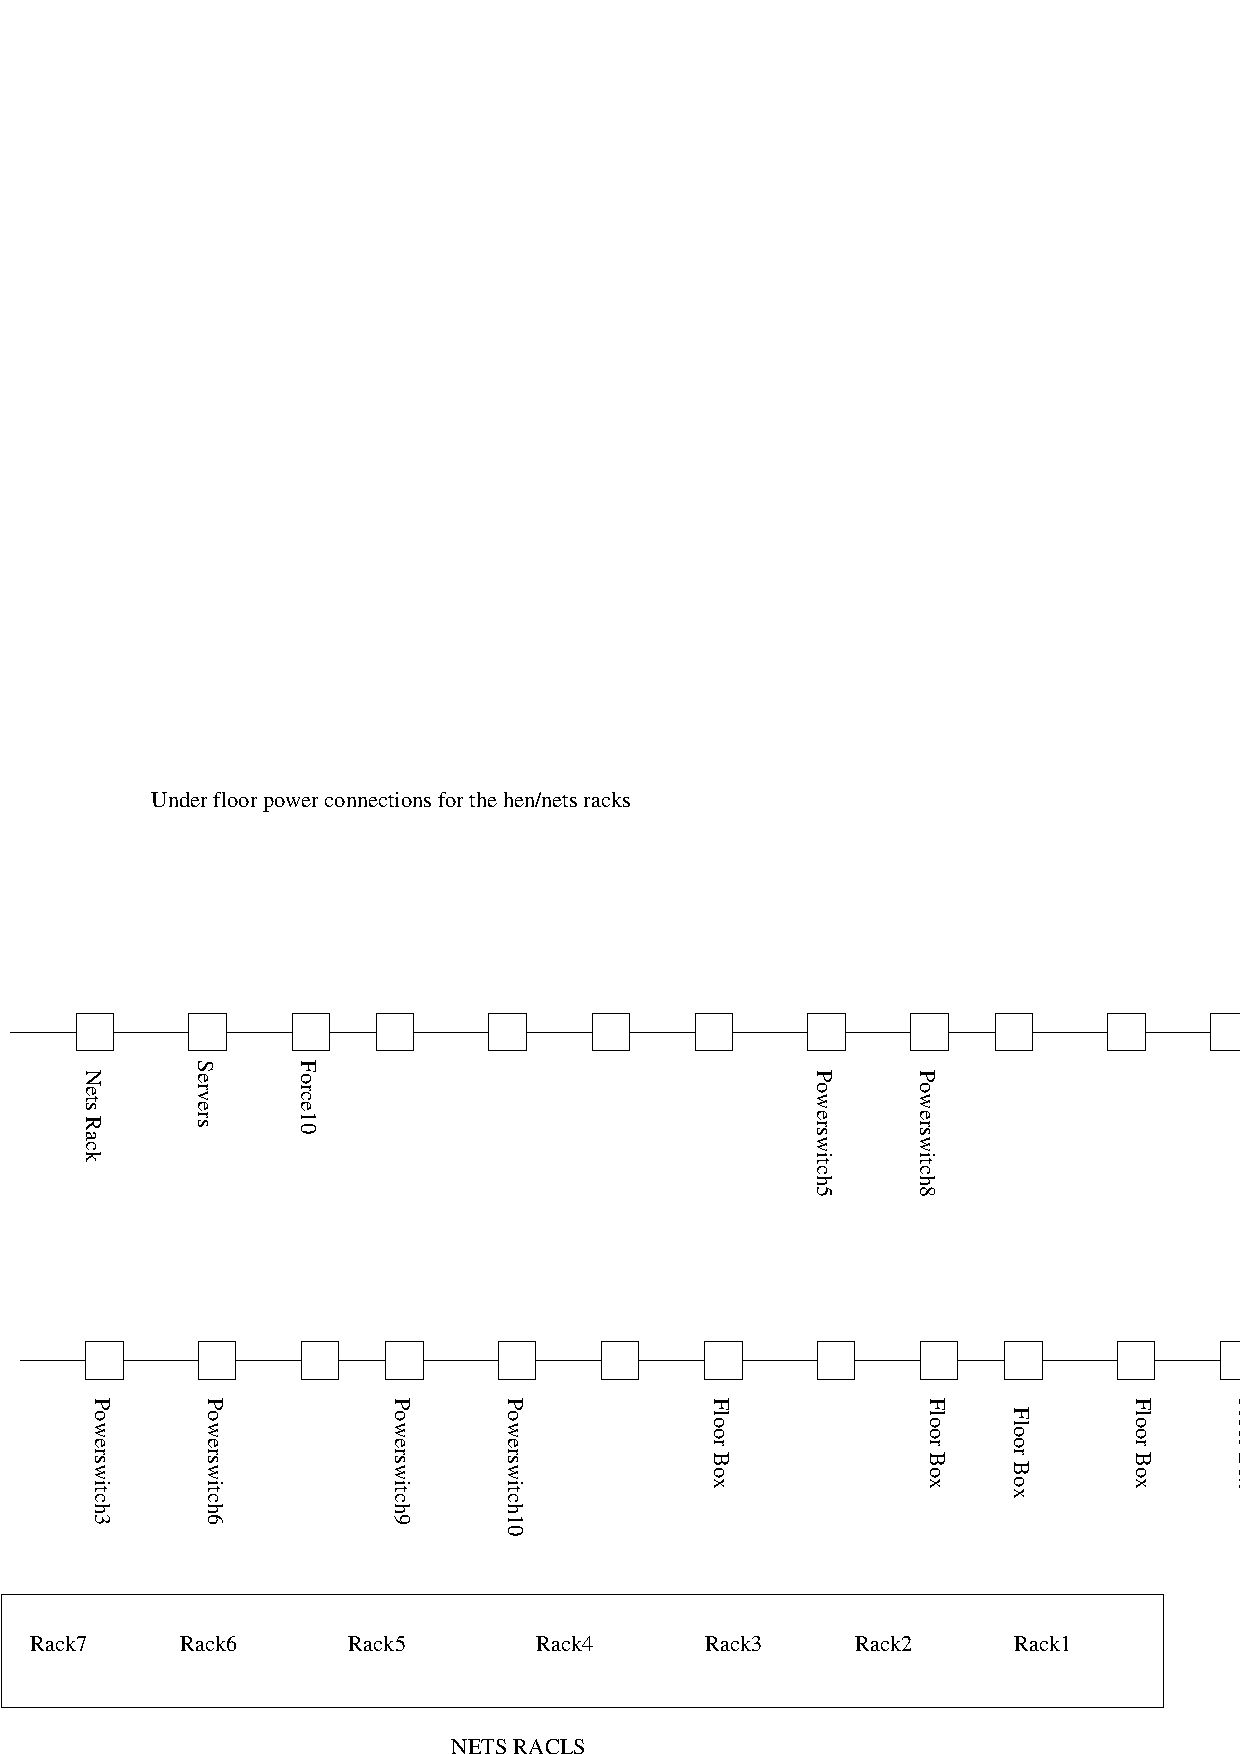
\includepdf[nup=1x1, landscape, 
  column=false,pages=1,addtotoc={1,subsection,2,underfloor wiring,},
  pagecommand={\thispagestyle{headings}}]{underfloor/underfloor.pdf}

\end{document}
